%
\section{Nützliches und Wissenswertes zum Erstellen einer Seminarausarbeitung}
\label{sec_stil}

\subsection{Allgemeine Hinweise}
Ganz allgemein handelt es sich bei der Seminarausarbeitung bereits um eine (richtige) {\bf wissenschaftliche Arbeit}.
Begehen Sie nicht den Fehler und sehen Sie diese als wortwörtliche Wiedergabe Ihres Seminarvortrags an, sondern beachten Sie stets die folgenden Punkte:
\begin{itemize}
\item Die sprachliche Darstellung der Ausarbeitung sollte dem Rahmen angepasst sein und stets auf einer sachlichen Argumentationsebene rangieren.
\item Der Schreibstil sollte unpersönlich gehalten werden. 
Vermeiden Sie Sätze, die die Wörter "`wir"', "`uns"', "`Sie"' usw.~enthalten.\footnote{Eine Ausnahme von dieser Regel stellen persönliche Kommentare, Bewertungen oder Urteile von Sachverhalten dar. Hier sollte klar werden, dass es sich um Ihre eigene Leistung handelt.}
\item Vermeiden Sie (Bandwurm-)Sätze, die sich über mehr als 2--3 Zeilen ziehen. Sie erhöhen damit signifikant die Lesbarkeit und die Verständlichkeit  Ihrer Arbeit.
\item Vermeiden Sie sprachliche Komplexität, d.h. beschränken Sie die Anzahl der notwendigen Nebensätze auf ein Mindestmaß.
\item Drücken Sie sich einfach und präzise aus. Vermeiden Sie eine \glqq geschraubte\grqq\, Ausdrucksweise.
\item Achten Sie auf temporale Konsistenz in der Verwendung von Präsens oder Präteritum  bei Verben.
\item Vermeiden Sie Worthülsen und unnötige Redewendungen ohne signifikanten Inhalt. 
\item Legen Sie Ihren Standpunkt stets mit der angemessenen Objektivität dar, auch wenn es um die Bewertung von Vor- oder Nachteilen des jeweiligen Themengegenstandes geht.
\item Vermeiden Sie unnötige Anglizismen (z.B.~"`connecten, downloaden, backupen"').
Existiert in diesem Zusammenhang bereits eine deutsche Redewendung, dann benutzen Sie diese (z.B. "`öffentlicher Schlüssel"' statt "`public key"').
Verwenden Sie englische Begriffe, so passen Sie diese entsprechend den deutschen Rechtschreibregeln bez.~Flexion, Silbentrennung, Getrennt- und Zusammenschreibung an.
\item Wenn Sie Begriffe einführen bzw. verwenden, deren Bedeutung nicht unmittelbar auch einem Nichtfachmann geläufig ist, sollten diese stets erläutert werden. 
Die Fachbegriffe sollten unmittelbar im Text erklärt werden. 
In natur- und. ingenieurwissenschaftlichen Arbeiten ist es eher unüblich, Erklärungen in Fußnoten zu platzieren. 
\item Achten Sie auf einen {\bf logischen Aufbau} Ihrer Arbeit, sowie ihrer einzelnen Unterkapitel und Gliederungspunkte.
\item {\bf Dringende Empfehlung:} Lassen Sie Ihre Ausarbeitung am besten von einem "`Nichtfachmann"'/einer "`Nichtfachfrau"', also nicht von einem Informatiker/einer Informatikerin korrekturlesen.
Auf diese Weise werden Schwachstellen in Ihrer Argumentation und andere logische Mängel in Ihrer Darstellung schnell deutlich.
\item Verwenden Sie konsequent die {\bf neue deutsche Rechtschreibung}.
Lassen Sie Ihren Text von einem Rechtschreibprogramm prüfen.
Allerdings kann dieses nur die korrekte Schreibweise von Einzelwörtern und (meist) nicht die korrekte Verwendung von Einzelwörtern im Satzzusammenhang überprüfen, insbesondere wenn es um grammatikalische Fehler oder Kommasetzung geht.
Verlassen Sie sich daher nicht alleine auf das Programm.
\item In deutschen Texten werden anstelle der englischen ''Quotes'' die Anführungsstriche in Form von "`Gänsefüßchen"' geschrieben. 
In dem Textsatzsystem {\LaTeX} stehen hierfür z.B. die Befehle \verb|\glqq| und \verb|\grqq| zur Verfügung. \\
{\bf Achtung:} Dazu muss das Paket {\tt ngerman} in den Header eingebunden werden.
\end{itemize}



\subsection{Weitere Formatierungshinweise}
\subsubsection{Abbildungen}
Abbildungen sind für das Erläutern und zum Verdeutlichen von komplexen Strukturen und Abläufen, wie sie üblicherweise in wissenschaftlichen Arbeiten beschrieben werden, unverzichtbar.
Die Abbildungen in Ihrer Arbeit sind stets zu {\bf nummerieren} und wie folgt zu setzen (siehe Abb.~\ref{fig_Abb1}).
%Hier eine Abbildung
\begin{figure}[ht]
  \begin{center}
  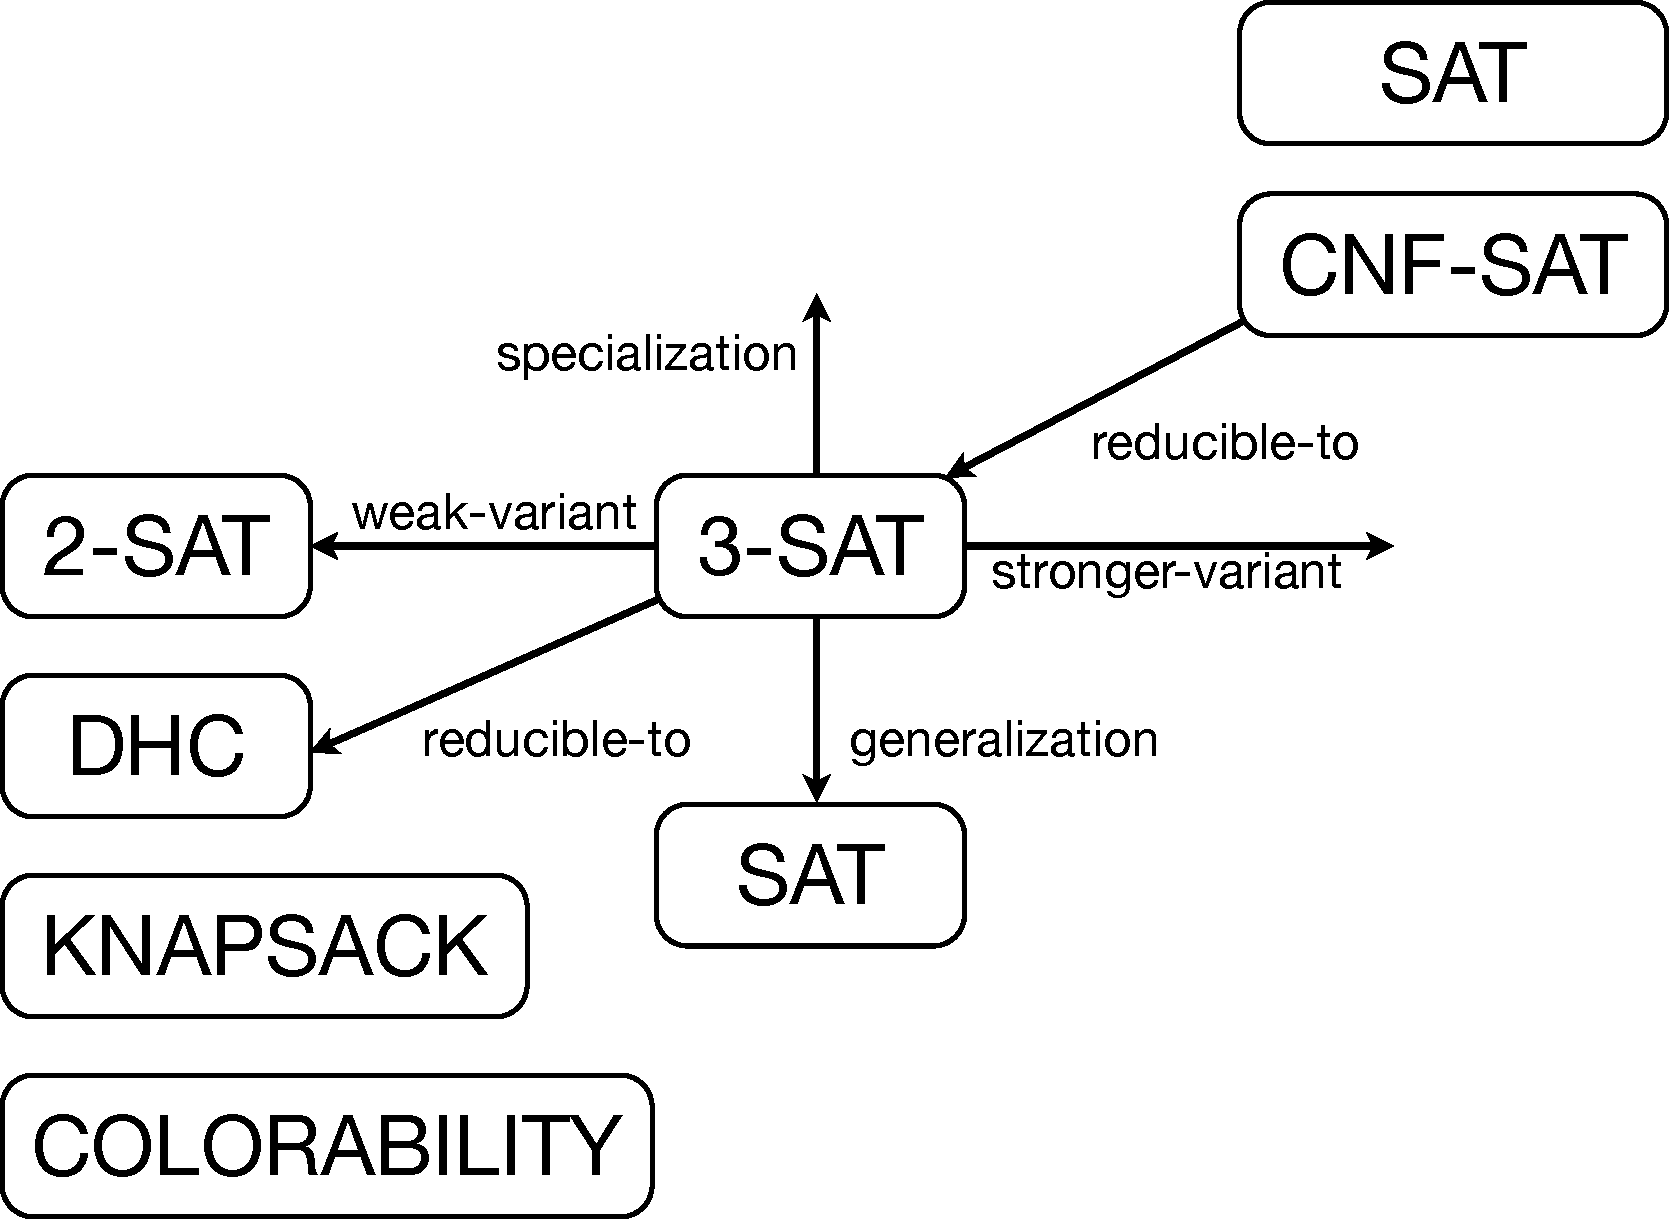
\includegraphics[width=0.5\textwidth]{images/3sat.pdf}
  \end{center}
  \caption{Das Umfeld des 3-SAT Problems}
  \label{fig_Abb1}
\end{figure} 

Jede Abbildung soll neben einer Abbildungsnummer eine Bildunterschrift ("`Das Umfeld des 3-SAT Problems"') besitzen, die die Grafik näher erläutert.
Weiterhin ist darauf zu achten, dass zu jeder Abbildung eine explizite Bezugnahme im Text aufgenommen wird, d.h. an geeigneter Stelle sollte ein Verweis der Form (siehe Abb.~\dots) erfolgen.

Beachten Sie bitte, dass es sich bei der vorliegenden Grafik um eine .eps-Datei handelt (Encapsulated Postscript), die mit Hilfe des \LaTeX-Pakets {\tt epsfig} eingebunden wurde.
Die Abbildung kann natürlich auch mit Hilfe anderer Pakete eingebunden werden, wie z.B. via {\tt graphicx} für .pdf-Dokumente.
Achten Sie dabei aber stets auf eine für den Druck geeignete Bildqualität!

\smallskip

\begin{center}
\colorbox{lightgray}{
\parbox{140mm}{
{\bf Achtung:} \\
Eine Abbildung sollte nicht einfach per "`copy and paste"' aus dem WWW in Ihre Ausarbeitung übernommen werden. 
Einerseits leidet im Allgemeinen bei einer solchen Vorgehensweise die Qualität bei einer entsprechenden Vergrößerung für die Druckaufbereitung stark darunter (siehe Abb.~\ref{fig_Abb2}), anderseits muss sichergestellt werden, dass der Urheber der Originalgrafik damit einverstanden ist, dass die Grafik in die Seminararbeit aufgenommen wird.
Der sicherste Weg ist deshalb, die Grafik mit einem geeigneten Grafikprogramm {\em selbst} zu erzeugen und anschließend in den Text einzubinden.}}
\end{center}

%Hier eine Abbildung
\begin{figure}[ht]
  \begin{center}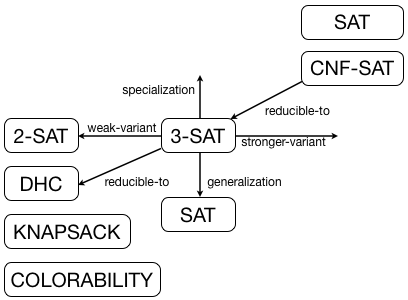
\includegraphics[width=0.5\textwidth]{images/3sat.png}\end{center}
  \caption{So sollte eine Abbildung nicht aussehen (JPG-Grafik, "`copy and paste"')}
  \label{fig_Abb2}
\end{figure} 
Verwenden Sie eine Abbildung, die in dieser Form bzw. in einer sehr ähnlichen Form bereits veröffentlicht wurde, müssen Sie dies durch eine bibliografische Referenz deutlich machen, d.h. Sie müssen wie bei einem Zitat die Fundstelle im Text als Literaturangabe aufnehmen.



\subsubsection{Tabellen}
Für Tabellen gilt dasselbe wie für Abbildungen.
Setzen Sie Tabellen nie in den Fließtext, sondern in die entsprechende \LaTeX-Tabellenumgebung und versehen Sie diese ebenfalls mit einer {\em Tabellennummer} und einer Tabellen{\em überschrift} (siehe Tabelle \ref{tab_HistoryWWW}).

%Hier eine Tabelle
\begin{table}
\caption{Die Geschichte des World Wide Web}
\begin{tabular}{rp{12cm}} \noalign{\smallskip} \hline \noalign{\smallskip}
{\bf 1945} & Vennevar Bush beschreibt MEMEX: das erste Hypertextsystem.\\
{\bf 1965} & Ted Nelson prägt als erster das Wort {\bf Hypertext} auf der ACM-Jahreskonferenz.\\ 
{\bf 1968} & Doug Engelbart entwickelt ein Hypertext-basiertes Prototypensystem NLS und erfindet zu diesem Zweck die Maus als Eingabegerät.\\
{\bf 1980} & Tim Berners Lee schreibt ein erste Notizbuch-Programm mit Hypertextlinks.\\
{\bf 1989} & Tim Berners Lee verfasst ein erstes Memorandum zu seinem Hypertext-Dokumentenverwaltungssystem am Kernforschungszentrum CERN.\\
{\bf 1990} & Zusammen mit Robert Cailliau entwickelt Tim Berners Lee den ersten WWW-Server und WWW-Browser: die Geburtsstunde des WorldWideWeb.\\  \noalign{\smallskip} \hline
\end{tabular}
\label{tab_HistoryWWW}
\end{table}  

\noindent
Grundsätzlich sollte man bei dem Setzen einer Tabelle sparsam mit grafischen Elementen -- wie Hilfslinien oder bunte Tabellenunterlegungen -- umgehen, da diese die Lesbarkeit sehr stark beeinträchtigen können.


\subsubsection{Listings, Quellcode und Pseudocode}

Sollten Sie Quellcode eines Programmes mit in Ihre Arbeit aufnehmen oder einen Algorithmus mit Hilfe von Pseudocode veranschaulichen, sind diese im Sinne einer Abbildung (siehe Abb.~\ref{fig_Abb3}) zu behandeln.
Ebenso wie eine Abbildung sind Listings, Quellcode oder Pseudocode jeweils mit einer laufenden Nummer und einer Bildunterschrift zu versehen.

\begin{figure}[ht]
\lstset{language=c++}
\lstset{backgroundcolor=\color{lightgray}}
\begin{lstlisting}{}
    for( i = 0; i < 10; i++ )
    {
        for( j = 0; j < 10; j++ )
        {
            // calculate $a_{ij}$
            a[i][j] = b[j][i];
        }
    }

\end{lstlisting}
  \caption{Einbinden von Quellcode in die Arbeit}
  \label{fig_Abb3}
\end{figure}

Sie können Listings z.B. mit Hilfe des \LaTeX-Pakets {\tt listings} einbinden.
Insbesondere, wenn längere Quellcode-Passagen in den Text eingebunden werden sollen, empfiehlt sich diese Vorgehensweise, da das Paket automatisch Seitenumbrüche korrekt formatiert und auch die Verwendung von internen Zeilennummern ermöglicht.

\subsubsection{Mathematische Formeln}

{\LaTeX} bietet sich insbesondere als Textverarbeitungssystem an, wenn es um das korrekte Formatieren mathematischer Ausdrücke und Formeln geht.
Versehen Sie alle Formeln, die Sie in Ihrer Arbeit verwenden -- insbesondere diejenigen, auf die Sie später noch Bezug nehmen --  mit einer entsprechenden Nummerierung.

\begin{equation}\label{formel1}
\frac{\sum_{n > 0} z^n}
{\prod_{1\leq k\leq n} (1-q^k)}
\end{equation}


\subsubsection{{\LaTeX} und andere Textverarbeitungssysteme}
Wenn Sie das Textsatzsystem {\LaTeX} für die Erstellung der Ausarbeitung verwenden, dann benutzen Sie das vorliegende \LaTeX-Musterdokument als Layoutvorlage für Ihre Arbeit.
Sollten Sie ein anderes Textverarbeitungsprogramm als {\LaTeX} verwenden, dann halten Sie sich bitte an die in diesem Beispieldokument verwendeten Bemaßungen und Formatierungen.
Sie können sich z.B.~dieses Beispieldokument ausdrucken und die entsprechenden Maßangaben, wie 
\begin{itemize}
\item linker, rechter Rand
\item Abstand oben, unten
\item etc.
\end{itemize}
abmessen und in Ihrem eigenen Textverarbeitungsprogramm verwenden. \\
Denken Sie bitte daran, dass neben einer gedruckten Version Ihrer Seminarausarbeitung auch eine {\bf pdf}-Datei abzugeben ist.
Diese können Sie zusammen mit Ihrer Präsentation (pdf-Datei + evtl.~ppt-Datei) via E-Mail zusenden.
